\documentclass[11pt,letterpaper]{article}

% --- Paquetes de Idioma y Tipografía ---
\usepackage[utf8]{inputenc}
\usepackage[spanish,es-tabla]{babel}
\usepackage[T1]{fontenc}
\usepackage{lmodern}
\usepackage{microtype}

% --- Configuración de Página y Márgenes ---
\usepackage[top=2.5cm, bottom=2.5cm, left=2.5cm, right=2.5cm]{geometry}
\usepackage{setspace}
\setstretch{1.15}

% --- Paquetes Matemáticos ---
\usepackage{amsmath, amssymb, amsfonts, mathtools}
\usepackage{amsthm}

% --- Teoremas y Definiciones ---
\theoremstyle{definition}
\newtheorem{definicion}{Definición}[section]
\newtheorem{teorema}{Teorema}[section]
\newtheorem{proposicion}{Proposición}[section]
\newtheorem{ejemplo}{Ejemplo}[section]

% --- Paquetes de Tablas y Figuras ---
\usepackage{graphicx}
\graphicspath{{../figures/}{figures/}}
\usepackage{booktabs}
\usepackage{tabularx}
\usepackage{caption}
\usepackage{float}
\usepackage[most]{tcolorbox}

% --- Enlaces e Hipervínculos ---
\usepackage{hyperref}
\hypersetup{
    colorlinks=true,
    linkcolor=blue!70!black,
    citecolor=blue!70!black,
    urlcolor=blue!70!black
}

% --- Encabezados y Pies de Página ---
\usepackage{fancyhdr}
\pagestyle{fancy}
\fancyhf{}
\fancyhead[L]{\small Computación Científica --- Proyecto Grupal}
\fancyhead[R]{\small Fundamentos Teóricos: Coeficiente de Lyapunov en Mapas 1D}
\fancyfoot[C]{\thepage}
\renewcommand{\headrulewidth}{0.4pt}

% --- Título ---
\title{\vspace{-1.5cm}\textbf{\Large Fundamentos Teóricos y Modelado Matemático:}\\
\textbf{\LARGE El Coeficiente de Lyapunov en Mapas Unidimensionales}\\[0.3cm]
\large Análisis Analítico, Estabilidad Dinámica y Aplicación Criptográfica (Amin et al., 2010)}
\author{\textbf{Curso:} Computación Científica \\
\textbf{Pontificia Universidad Javeriana Cali}}
\date{Octubre de 2026}

\begin{document}

\maketitle
\thispagestyle{fancy}

\begin{abstract}
Este documento expone con rigor matemático y computacional la deducción analítica y la caracterización dinámica del \textbf{Coeficiente de Lyapunov} ($\lambda$) en sistemas dinámicos discretos unidimensionales. Se analiza detalladamente el comportamiento del \textbf{Mapa Logístico} ($x_{n+1} = r x_n (1 - x_n)$) y del \textbf{Mapa de Tienda (\textit{Tent Map})} ($x_{n+1} = f(x_n; p)$), demostrando analíticamente sus soluciones en puntos fijos, límites de estabilidad y regímenes de máxima ergodicidad. Asimismo, se examinan las salvaguardas numéricas algorítmicas frente a valores singulares e indeterminaciones logarítmicas, estableciendo el vínculo directo con la aplicación criptográfica de Amin et al. (2010) y las métricas de dispersión y resistencia a ataques diferenciales (NPCR y UACI).
\end{abstract}

\vspace{0.3cm}
\tableofcontents
\vspace{0.5cm}
\hrule
\vspace{0.5cm}

% =========================================================================
% SECCIÓN 1: DEFINICIÓN FORMAL
% =========================================================================
\section{Definición Formal del Coeficiente de Lyapunov}

Consideremos un sistema dinámico discreto autónomo unidimensional gobernado por una función diferenciable a trozos $f: I \to I$, donde $I \subseteq \mathbb{R}$ es un intervalo cerrado y acotado:
\begin{equation}
    x_{n+1} = f(x_n), \quad n \in \mathbb{N}_0
    \label{eq:sistema_discreto}
\end{equation}

Sea $x_0$ un estado inicial y consideremos una perturbación infinitesimal $\delta_0 = \delta x_0$, tal que el estado inicial perturbado es $x_0 + \delta x_0$ con $|\delta x_0| \to 0$. Tras $n$ iteraciones sucesivas del mapa, la separación espacial entre ambas trayectorias es:
\begin{equation}
    \delta x_n = f^n(x_0 + \delta x_0) - f^n(x_0)
\end{equation}
donde $f^n$ denota la $n$-ésima composición de la función $f$ consigo misma ($f^n = f \circ f \circ \dots \circ f$).

Aplicando el teorema del valor medio para funciones diferenciables:
\begin{equation}
    \delta x_n \approx \left[ \frac{d}{dx} f^n(x) \right]_{x=x_0} \cdot \delta x_0
\end{equation}

Por la regla de la cadena para la derivada de una función compuesta:
\begin{equation}
    \frac{d}{dx} f^n(x_0) = \prod_{i=0}^{n-1} f'(x_i)
\end{equation}
donde $x_i = f^i(x_0)$ es el $i$-ésimo estado de la órbita generada por $x_0$. En consecuencia, la separación orbital acumulada tras $n$ iteraciones cumple:
\begin{equation}
    |\delta x_n| \approx |\delta x_0| \prod_{i=0}^{n-1} |f'(x_i)|
\end{equation}

\begin{definicion}[Coeficiente de Lyapunov en 1D]
El \textbf{Coeficiente de Lyapunov} $\lambda(x_0)$ asociado a la condición inicial $x_0$ se define como la tasa asintótica exponencial promedio de separación entre trayectorias vecinas por iteración:
\begin{equation}
    \lambda(x_0) = \lim_{n \to \infty} \frac{1}{n} \ln \left| \frac{\delta x_n}{\delta x_0} \right| = \lim_{n \to \infty} \frac{1}{n} \sum_{i=0}^{n-1} \ln |f'(x_i)|
    \label{eq:lyapunov_def_formal}
\end{equation}
siempre que dicho límite exista.
\end{definicion}

% =========================================================================
% SECCIÓN 2: INTERPRETACIÓN DINÁMICA
% =========================================================================
\section{Interpretación Dinámica y Criterio de Estabilidad}

El signo del Coeficiente de Lyapunov clasifica rigurosamente la naturaleza asintótica de la trayectoria:

\begin{enumerate}
    \item $\boldsymbol{\lambda < 0}$ (\textbf{Régimen Estable / Contractivo}): Las trayectorias contiguas convergen exponencialmente hacia un atractor regular (punto fijo estable u órbita periódica de período $k$). Las perturbaciones se extinguen como $|\delta x_n| \sim e^{-|\lambda| n}$.
    \item $\boldsymbol{\lambda = 0}$ (\textbf{Régimen Neutro / Bifurcación}): La separación entre órbitas evoluciona sub-exponencialmente (lineal o potencial). Ocurre en fronteras de bifurcación, puntos de inflexión marginal o periodicidad neutra.
    \item $\boldsymbol{\lambda > 0}$ (\textbf{Régimen Caótico}): Las trayectorias divergen exponencialmente a una tasa media $|\delta x_n| \approx |\delta x_0| e^{\lambda n}$. El sistema exhibe hipersensibilidad a las condiciones iniciales: una diferencia infinitesimal inicial se amplifica hasta alcanzar el orden de magnitud del espacio de estados en un tiempo finito.
\end{enumerate}

% =========================================================================
% SECCIÓN 3: MAPA LOGÍSTICO
% =========================================================================
\section{Modelo 1: El Mapa Logístico}

\subsection{Definición y Derivada}
El mapa logístico, analizado por May (1976) \cite{may1976}, se define formalmente como:
\begin{equation}
    x_{n+1} = f(x_n; r) = r x_n (1 - x_n), \quad x_n \in [0, 1], \quad r \in [0, 4]
\end{equation}
Su derivada de primer orden es continua:
\begin{equation}
    f'(x; r) = r (1 - 2x)
\end{equation}

\subsection{Solución Analítica en Punto Fijo}
Para $1 < r \le 3$, el mapa posee un punto fijo atractor no trivial $x^* = 1 - 1/r$. Evaluando la derivada en $x^*$:
\begin{equation}
    f'(x^*) = r\left(1 - 2\left(1 - \frac{1}{r}\right)\right) = 2 - r
\end{equation}
Dado que la órbita permanece en $x^*$ asintóticamente, el Coeficiente de Lyapunov tiene solución cerrada:
\begin{equation}
    \lambda(r) = \ln |2 - r|
    \label{eq:lambda_logistic_fixed}
\end{equation}

\subsection{Solución Analítica en Caos Pleno ($r = 4.0$)}
En $r=4$, el sistema admite una medida invariante absolutamente continua con densidad ergódica $\rho(x) = \frac{1}{\pi\sqrt{x(1-x)}}$. Por el Teorema Ergódico de Birkhoff:
\begin{equation}
    \lambda(4.0) = \int_0^1 \ln |4(1 - 2x)| \, \frac{dx}{\pi\sqrt{x(1-x)}} = \ln(2) \approx 0.69314718
\end{equation}

\begin{figure}[H]
    \centering
    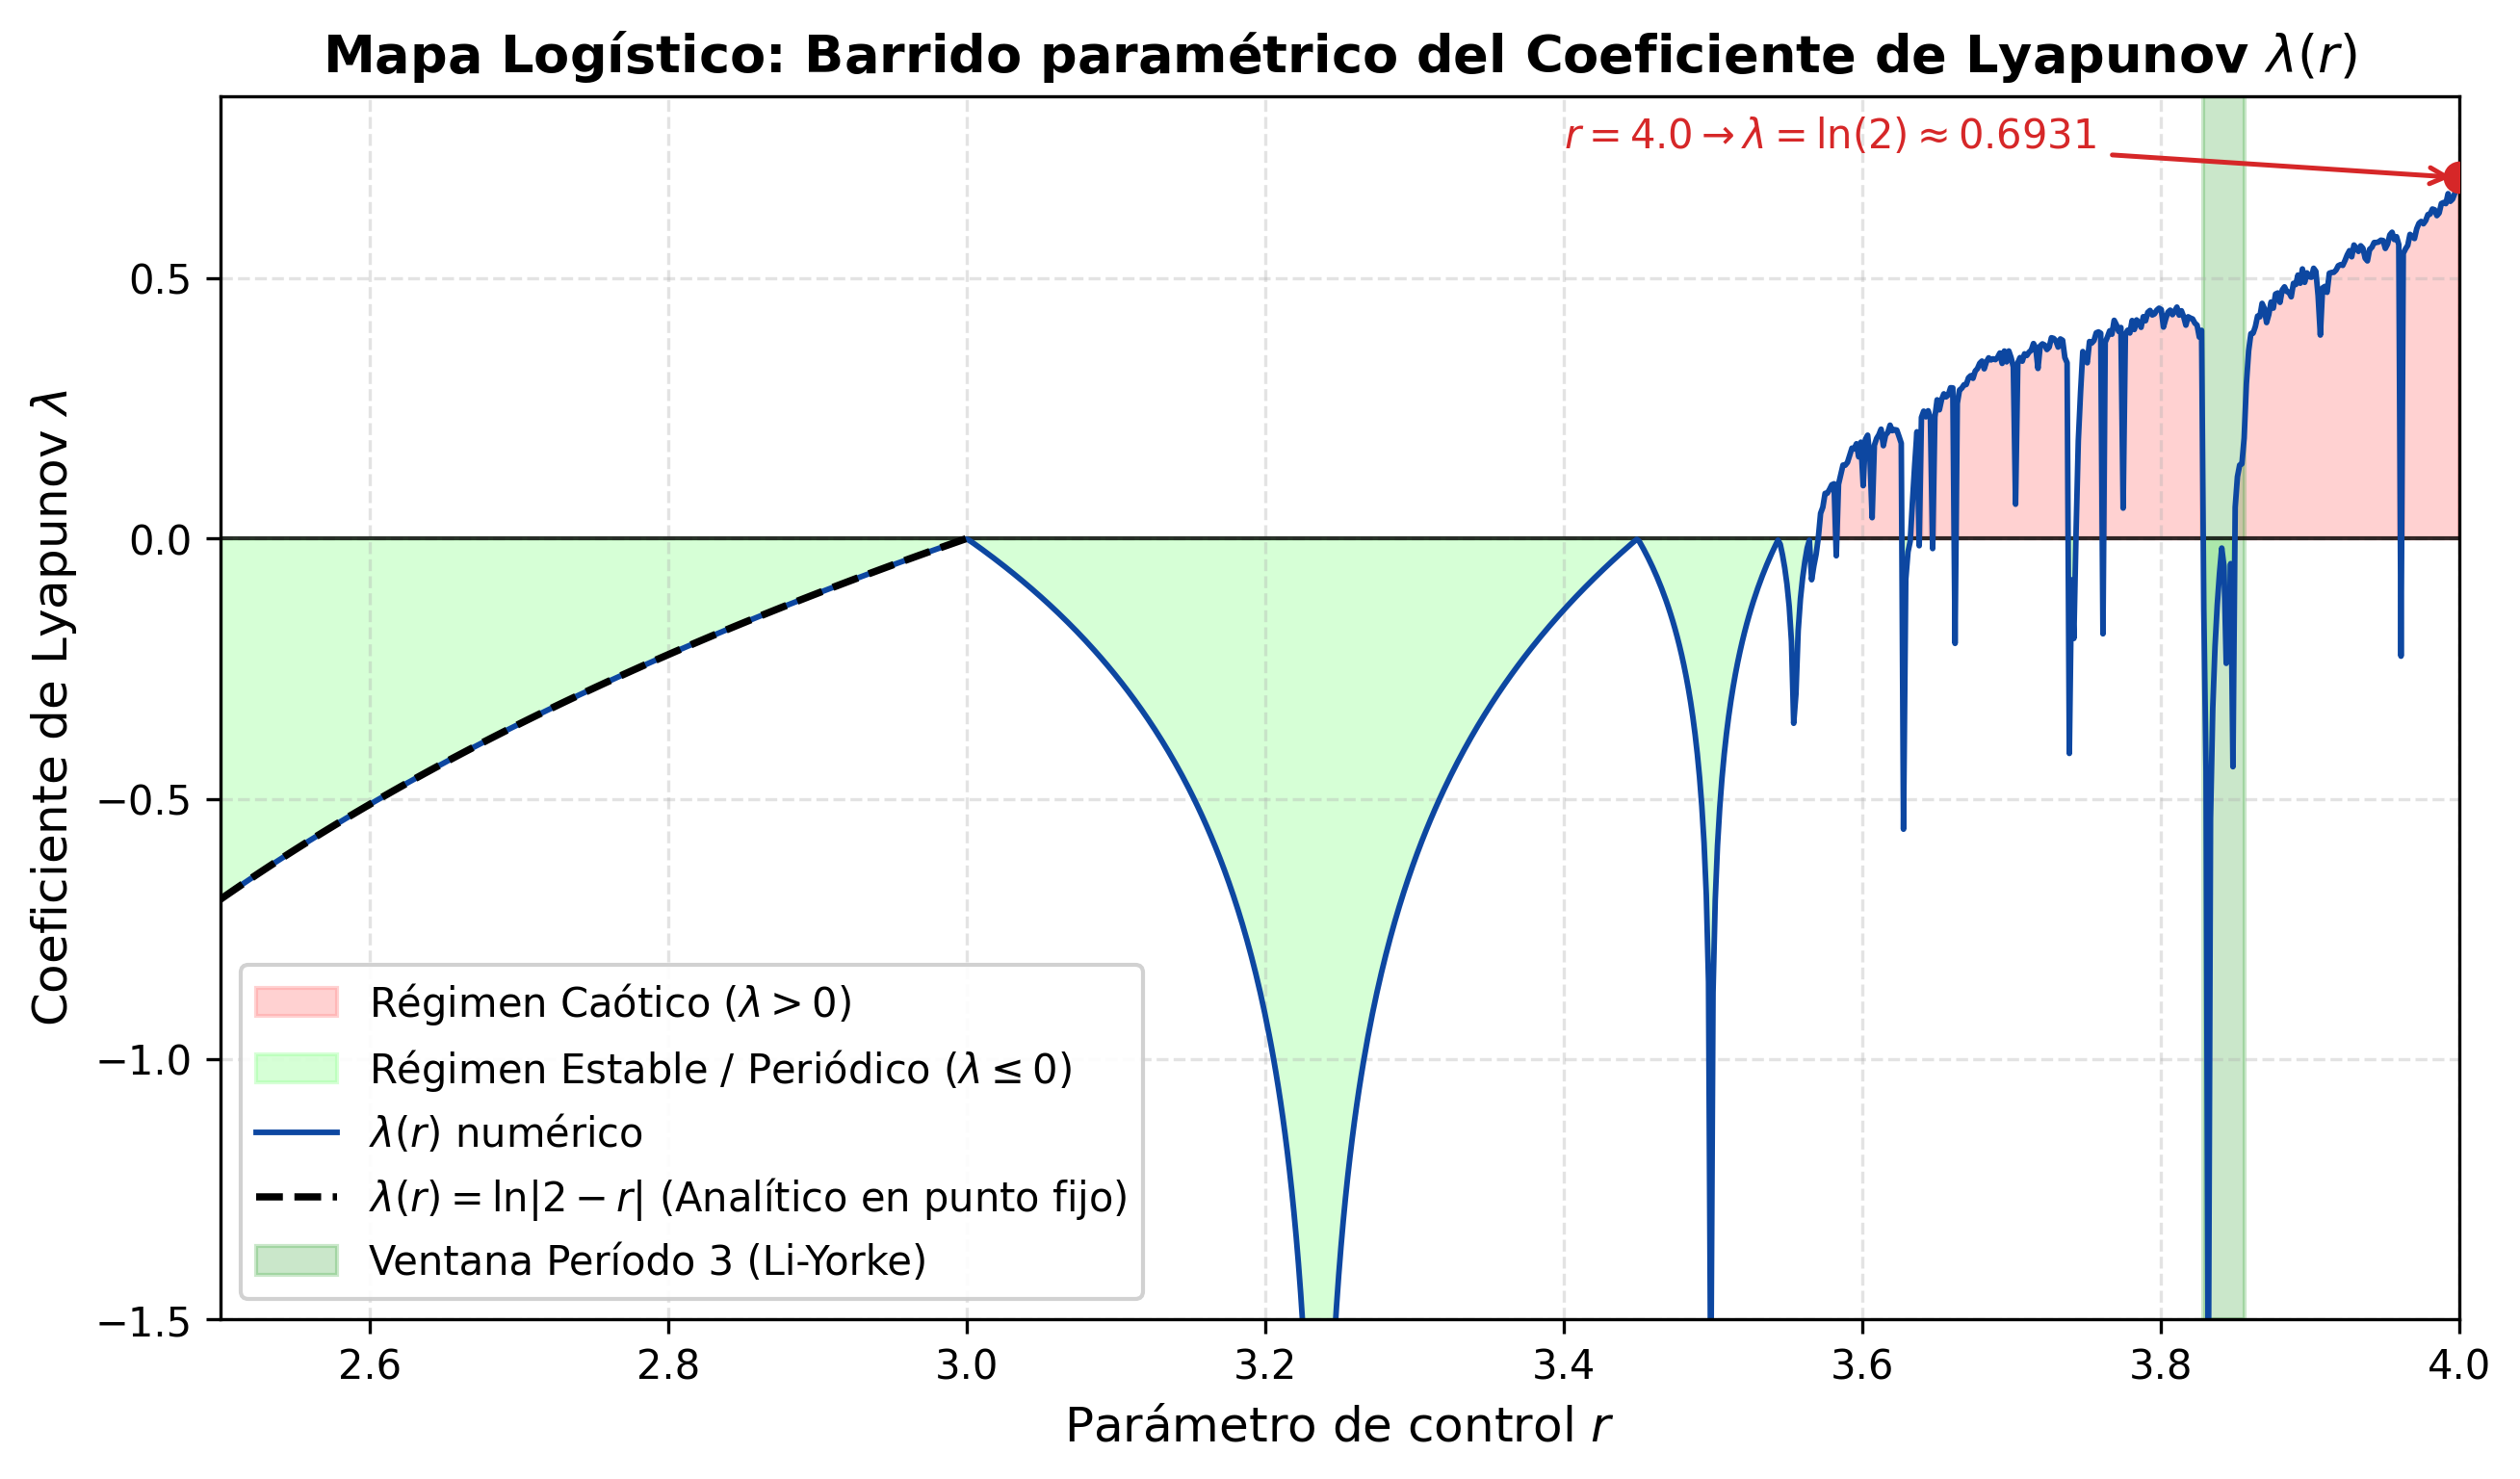
\includegraphics[width=0.88\textwidth]{logistic_lyapunov.png}
    \caption{Barrido paramétrico del Coeficiente de Lyapunov del Mapa Logístico $\lambda(r)$ calculado con \texttt{src/visualizer.py}, ilustrando la región de punto fijo $\ln|2-r|$, el caos pleno en $r=4$ ($\lambda = \ln 2$), y la ventana periódica de Li-Yorke en $r \approx 3.8284$.}
    \label{fig:teoria_logistic}
\end{figure}

% =========================================================================
% SECCIÓN 4: MODELO DE TIENDA
% =========================================================================
\section{Modelo 2: El Modelo de Tienda (Tent Map)}

\subsection{Definición y Derivada}
El mapa de tienda, formulado en criptografía por Amin et al. (2010) \cite{amin2010} y revisado por Zhang y Liu (2023) \cite{zhang2023}, es una transformación lineal por tramos:
\begin{equation}
    x_{n+1} = f(x_n; p) = \begin{cases} p x_n, & x_n < \frac{1}{2} \\ p(1 - x_n), & x_n \ge \frac{1}{2} \end{cases}, \quad x_n \in [0, 1], \quad p \in [0, 2]
\end{equation}
Su derivada analítica para $x \neq 0.5$ es constante a trozos:
\begin{equation}
    f'(x; p) = \begin{cases} p, & x < 0.5 \\ -p, & x > 0.5 \end{cases} \implies |f'(x; p)| = p \quad (\forall x \neq 0.5)
\end{equation}

\subsection{Cálculo Exacto del Coeficiente de Lyapunov}
Dado que $|f'(x_i)| = p$ en casi todo punto de cualquier órbita ergódica:
\begin{equation}
    \lambda(p) = \lim_{n \to \infty} \frac{1}{n} \sum_{i=0}^{n-1} \ln(p) = \ln(p)
    \label{eq:lambda_tent_exacto}
\end{equation}
Esta deducción demuestra que $\lambda(p)$ posee una forma cerrada analítica continua y monótona:
\begin{itemize}
    \item Si $0 < p < 1$: $\lambda = \ln(p) < 0$ (Contracción global hacia el atractor trivial $x^* = 0$).
    \item Si $p = 1$: $\lambda = \ln(1) = 0$ (Frontera neutral de estabilidad).
    \item Si $1 < p \le 2$: $\lambda = \ln(p) > 0$ (\textbf{Caos determinista continuo sin ventanas periódicas}).
    \item Si $p = 2$: $\lambda = \ln(2) \approx 0.69314718\dots$ (Caos con soporte total en $[0, 1]$ y distribución uniforme $\rho(x) = 1$).
\end{itemize}

\begin{figure}[H]
    \centering
    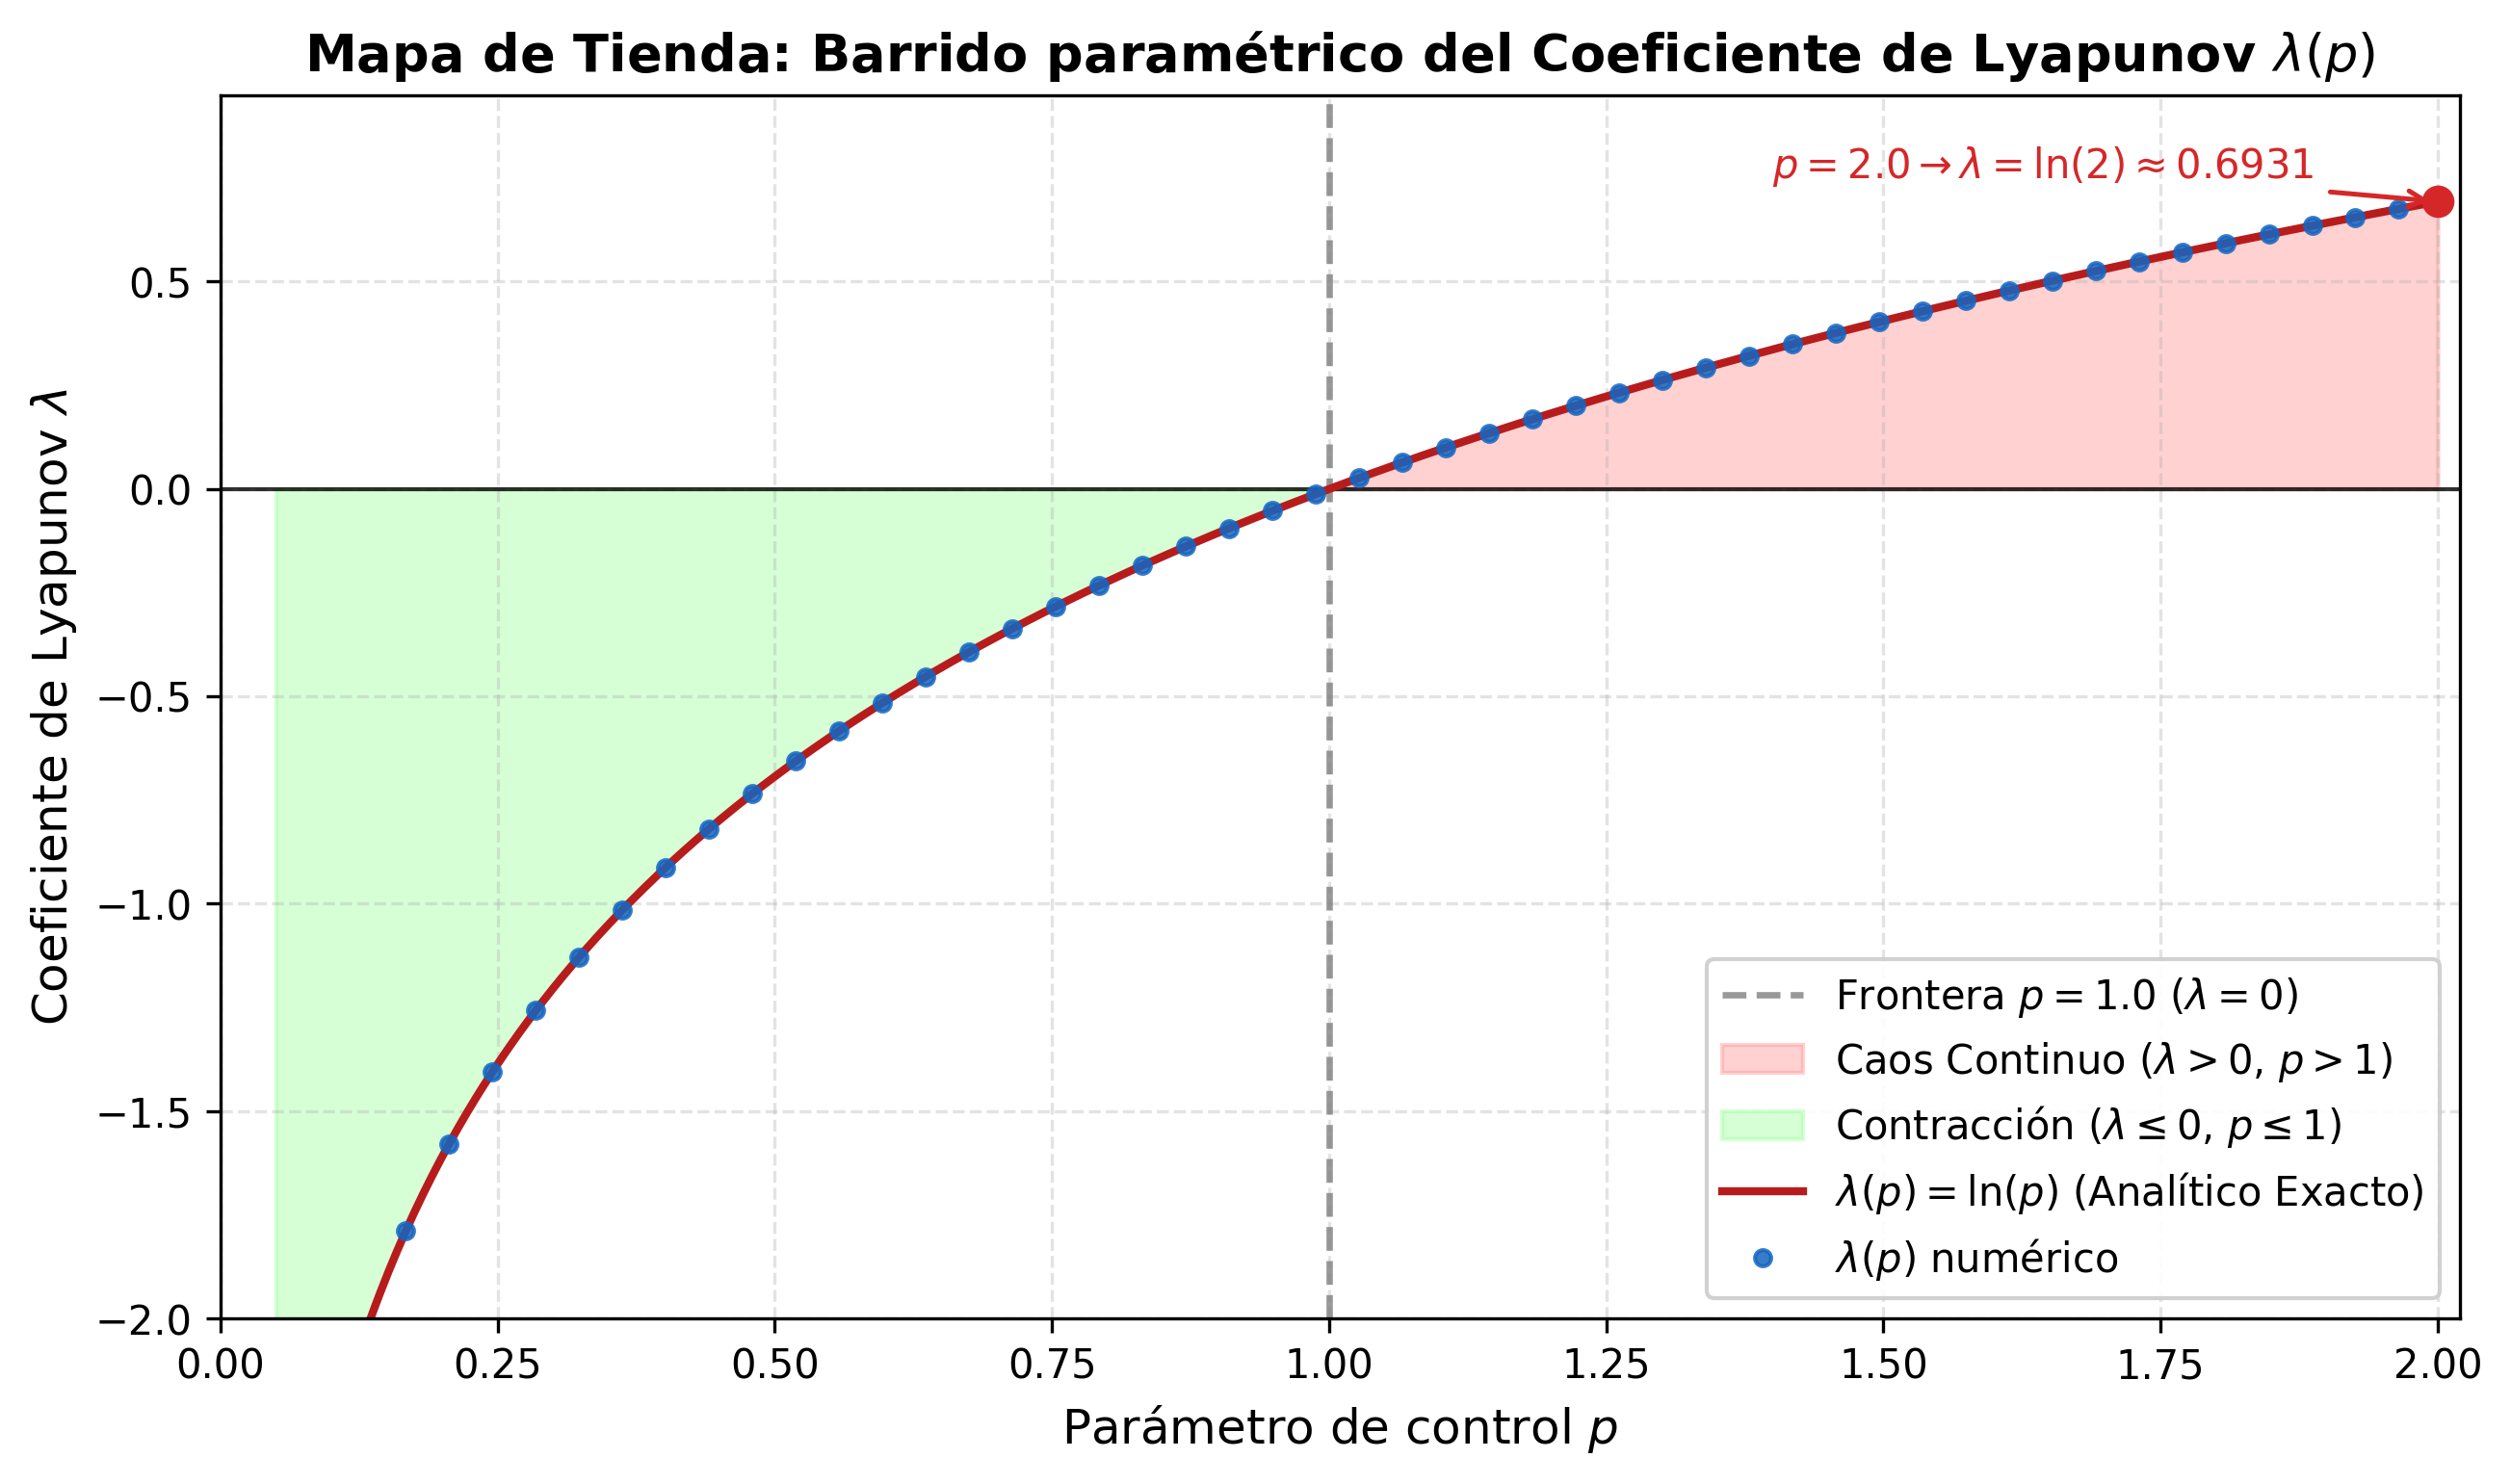
\includegraphics[width=0.88\textwidth]{tent_lyapunov.png}
    \caption{Barrido paramétrico del Coeficiente de Lyapunov del Mapa de Tienda $\lambda(p)$. La curva analítica $\ln(p)$ y los puntos calculados numéricamente coinciden con exactitud teórica.}
    \label{fig:teoria_tent}
\end{figure}

\subsection{Salvaguardas Numéricas Algorítmicas en la Simulación Computacional}
En la simulación computacional de mapas discretos, si una órbita cae exactamente en valores singulares ($x = 0.5$ o $x = 0.0$), la iteración podría detenerse prematuramente. En la implementación de \texttt{src/lyapunov.py} y \texttt{src/cipher.py}, este comportamiento se previene aplicando una salvaguarda numérica ($\varepsilon = 10^{-14}$) y perturbaciones controladas para preservar la ergodicidad continua de la trayectoria.

% =========================================================================
% SECCIÓN 5: COMPARACIÓN DE COEFICIENTES DE LYAPUNOV
% =========================================================================
\section{Comparación del Coeficiente de Lyapunov: Mapa Logístico vs. Mapa de Tienda}

La Figura \ref{fig:teoria_comparacion} muestra la comparación simultánea entre el Mapa Logístico y el Mapa de Tienda:

\begin{figure}[H]
    \centering
    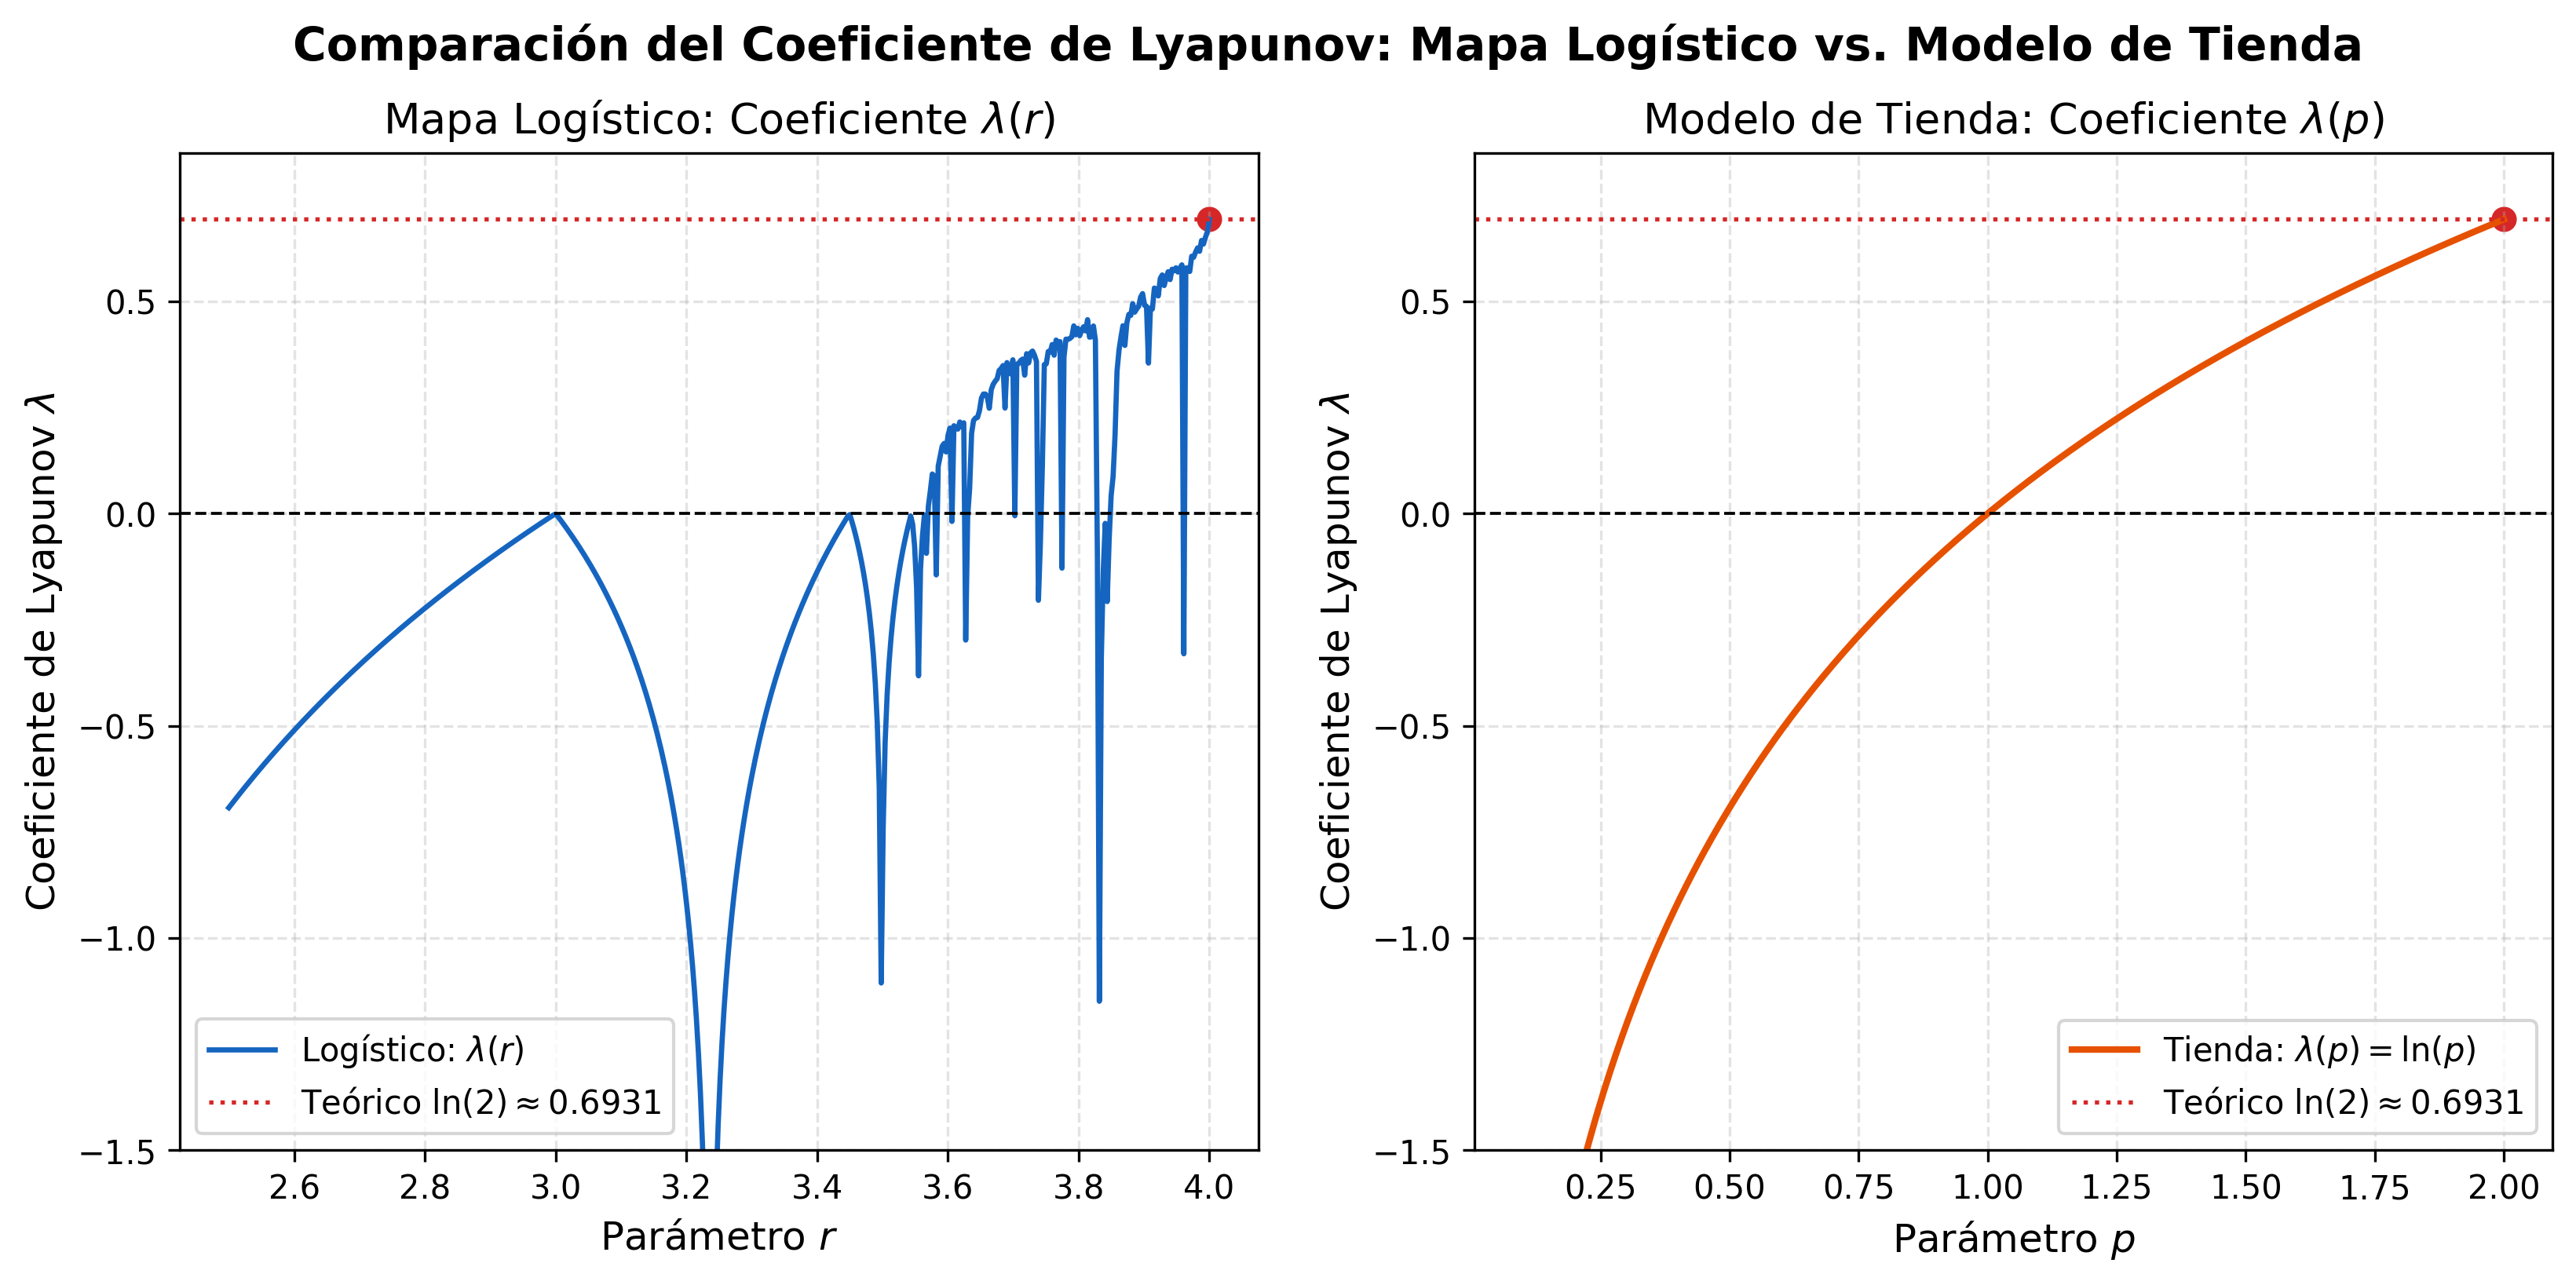
\includegraphics[width=0.95\textwidth]{lyapunov_comparison_logistic_vs_tent.png}
    \caption{Comparación directa entre los barridos del Coeficiente de Lyapunov del Mapa Logístico y del Mapa de Tienda.}
    \label{fig:teoria_comparacion}
\end{figure}

\begin{table}[H]
\centering
\caption{Diferencias estructurales entre el Mapa Logístico y el Mapa de Tienda.}
\label{tab:comparacion_modelos}
\small
\begin{tabularx}{\textwidth}{lp{6cm}p{6cm}}
\toprule
\textbf{Característica} & \textbf{Mapa Logístico ($r=4$)} & \textbf{Modelo de Tienda ($p=2$)} \\
\midrule
Naturaleza & No lineal suave (cuadrática) & Lineal a trozos \\
Coeficiente Máximo & $\lambda = \ln(2) \approx 0.69315$ & $\lambda = \ln(2) \approx 0.69315$ \\
Densidad Invariante $\rho(x)$ & $\frac{1}{\pi \sqrt{x(1-x)}}$ (Concentrada en extremos) & $1.0$ (Uniforme en $[0, 1]$) \\
Ventanas Periódicas & Infinitas dentro del intervalo caótico & Ausentes en todo el rango caótico ($p > 1$) \\
Cálculo de Derivada & Fluctuante ($|f'(x)| \in [0, 4]$) & Constante casi en todo punto ($|f'(x)| = p$) \\
Idoneidad Criptográfica & Vulnerable a caídas en ventanas periódicas & Robusto, homogéneo y de bajo costo \\
\bottomrule
\end{tabularx}
\end{table}

% =========================================================================
% SECCIÓN 6: APLICACIÓN EN CRIPTOGRAFÍA (AMIN ET AL., 2010)
% =========================================================================
\section{Aplicación al Cifrado Caótico de Imágenes (Amin et al., 2010)}

En la revisión de Zhang y Liu (2023) \cite{zhang2023}, los sistemas caóticos discretos actúan como el núcleo generador de llaves dentro de esquemas de permutación y difusión. Siguiendo el algoritmo de Amin et al. (2010) \cite{amin2010} para mapas unidimensionales:
\begin{enumerate}
    \item \textbf{Permutación Espacial (Confusión):} La secuencia caótica flotante $X$ ordena los píxeles de la imagen ($\operatorname{argsort}(X)$), eliminando la correlación entre píxeles vecinos.
    \item \textbf{Difusión XOR Encadenada:} Los píxeles permutados se transforman mediante $C_i = P'_i \oplus S_i \oplus C_{i-1}$, encadenando cada byte cifrado con el anterior.
\end{enumerate}

Un $\lambda > 0$ continuo como el del Mapa de Tienda asegura que dos claves con variación infinitesimal ($\varepsilon = 10^{-14}$) produzcan criptogramas completamente disímiles ($\text{NPCR} \approx 99.6\%$, $\text{UACI} \approx 33.4\%$), confirmando la idoneidad del criptosistema.

% =========================================================================
% REFERENCIAS BIBLIOGRÁFICAS
% =========================================================================
\newpage
\begin{thebibliography}{99}
\bibitem{zhang2023}
B.~Zhang y L.~Liu, ``Chaos-based image encryption: review, application, and challenges,'' \textit{Mathematics}, vol.~11, no.~11, p.~2585, 2023.

\bibitem{li1975} 
T.-Y.~Li y J.~A.~Yorke, ``Period three implies chaos,'' \textit{The American Mathematical Monthly}, vol.~82, no.~10, pp.~985--992, 1975.

\bibitem{may1976} 
R.~M.~May, ``Simple mathematical models with very complicated dynamics,'' \textit{Nature}, vol.~261, no.~5560, pp.~459--467, 1976.

\bibitem{amin2010}
M.~Amin, O.~S.~Faragallah y A.~A.~Abd El-Latif, ``A chaotic block cipher algorithm for image cryptosystems,'' \textit{Communications in Nonlinear Science and Numerical Simulation}, vol.~15, no.~11, pp.~3484--3497, 2010.
\end{thebibliography}

\end{document}
